\chapter{Background}\label{ch:backg}
In recent years, the IoT revolution has led to the creation of enormous amounts of data. The use of intelligent devices that can interface with cloud computing systems or perform complex calculations directly on board, in homes and cities, has allowed the affirmation of data-driven algorithms compared to other methodologies used so far. In fact, these approaches try to emulate the functioning of the human mind, enabling computers to perform tasks that are unthinkable until now. 
In this chapter are resumed the data-driven and machine learning algorithms used for developing the proposed methodologies for fall classification systems.

\section{Support Vector Machines}
Support Vector Machines (SVM) \cite{cortes95} are one of the most popular classification algorithms and are well known for their strong theoretical foundations, generalization performance and ability to handle high dimensional data.
This section presents an overview of support vector machine, starting with linear
SVMs, followed by their extension to the nonlinear case and finally the One-Class SVM for novelty detection.

\paragraph{Linear Support Vector Machines}
In the binary classification setting, let $((x_1, y_1)\dots(x_n, y_n))$ be the training dataset where $x_i \in \Re^n$ are the $n$-dimensional feature vectors representing the instances (i.e. observations) and  $y_i \in \{-1, +1\}$ be the labels of the instances. Support vector learning is the problem of finding a separating hyperplane that separates the positive examples (labeled +1) from the negative examples (labeled -1) with the largest margin:
\begin{equation}
f(\vec{w}) =  \mbox{sign} (\vec{w}^T \cdot \vec{x} + b),
\end{equation} 
where a value of $-1$ indicates one class, and a value of $+1$ the other class.
In the simpler linearly separable problem, the margin of the hyperplane is defined as the shortest distance between the positive and negative instances that are closest to the hyperplane. The intuition behind searching for the hyperplane with a large margin is that a hyperplane with the largest margin should be more resistant to noise than a hyperplane with a smaller margin.
\begin{figure}
	\centering
	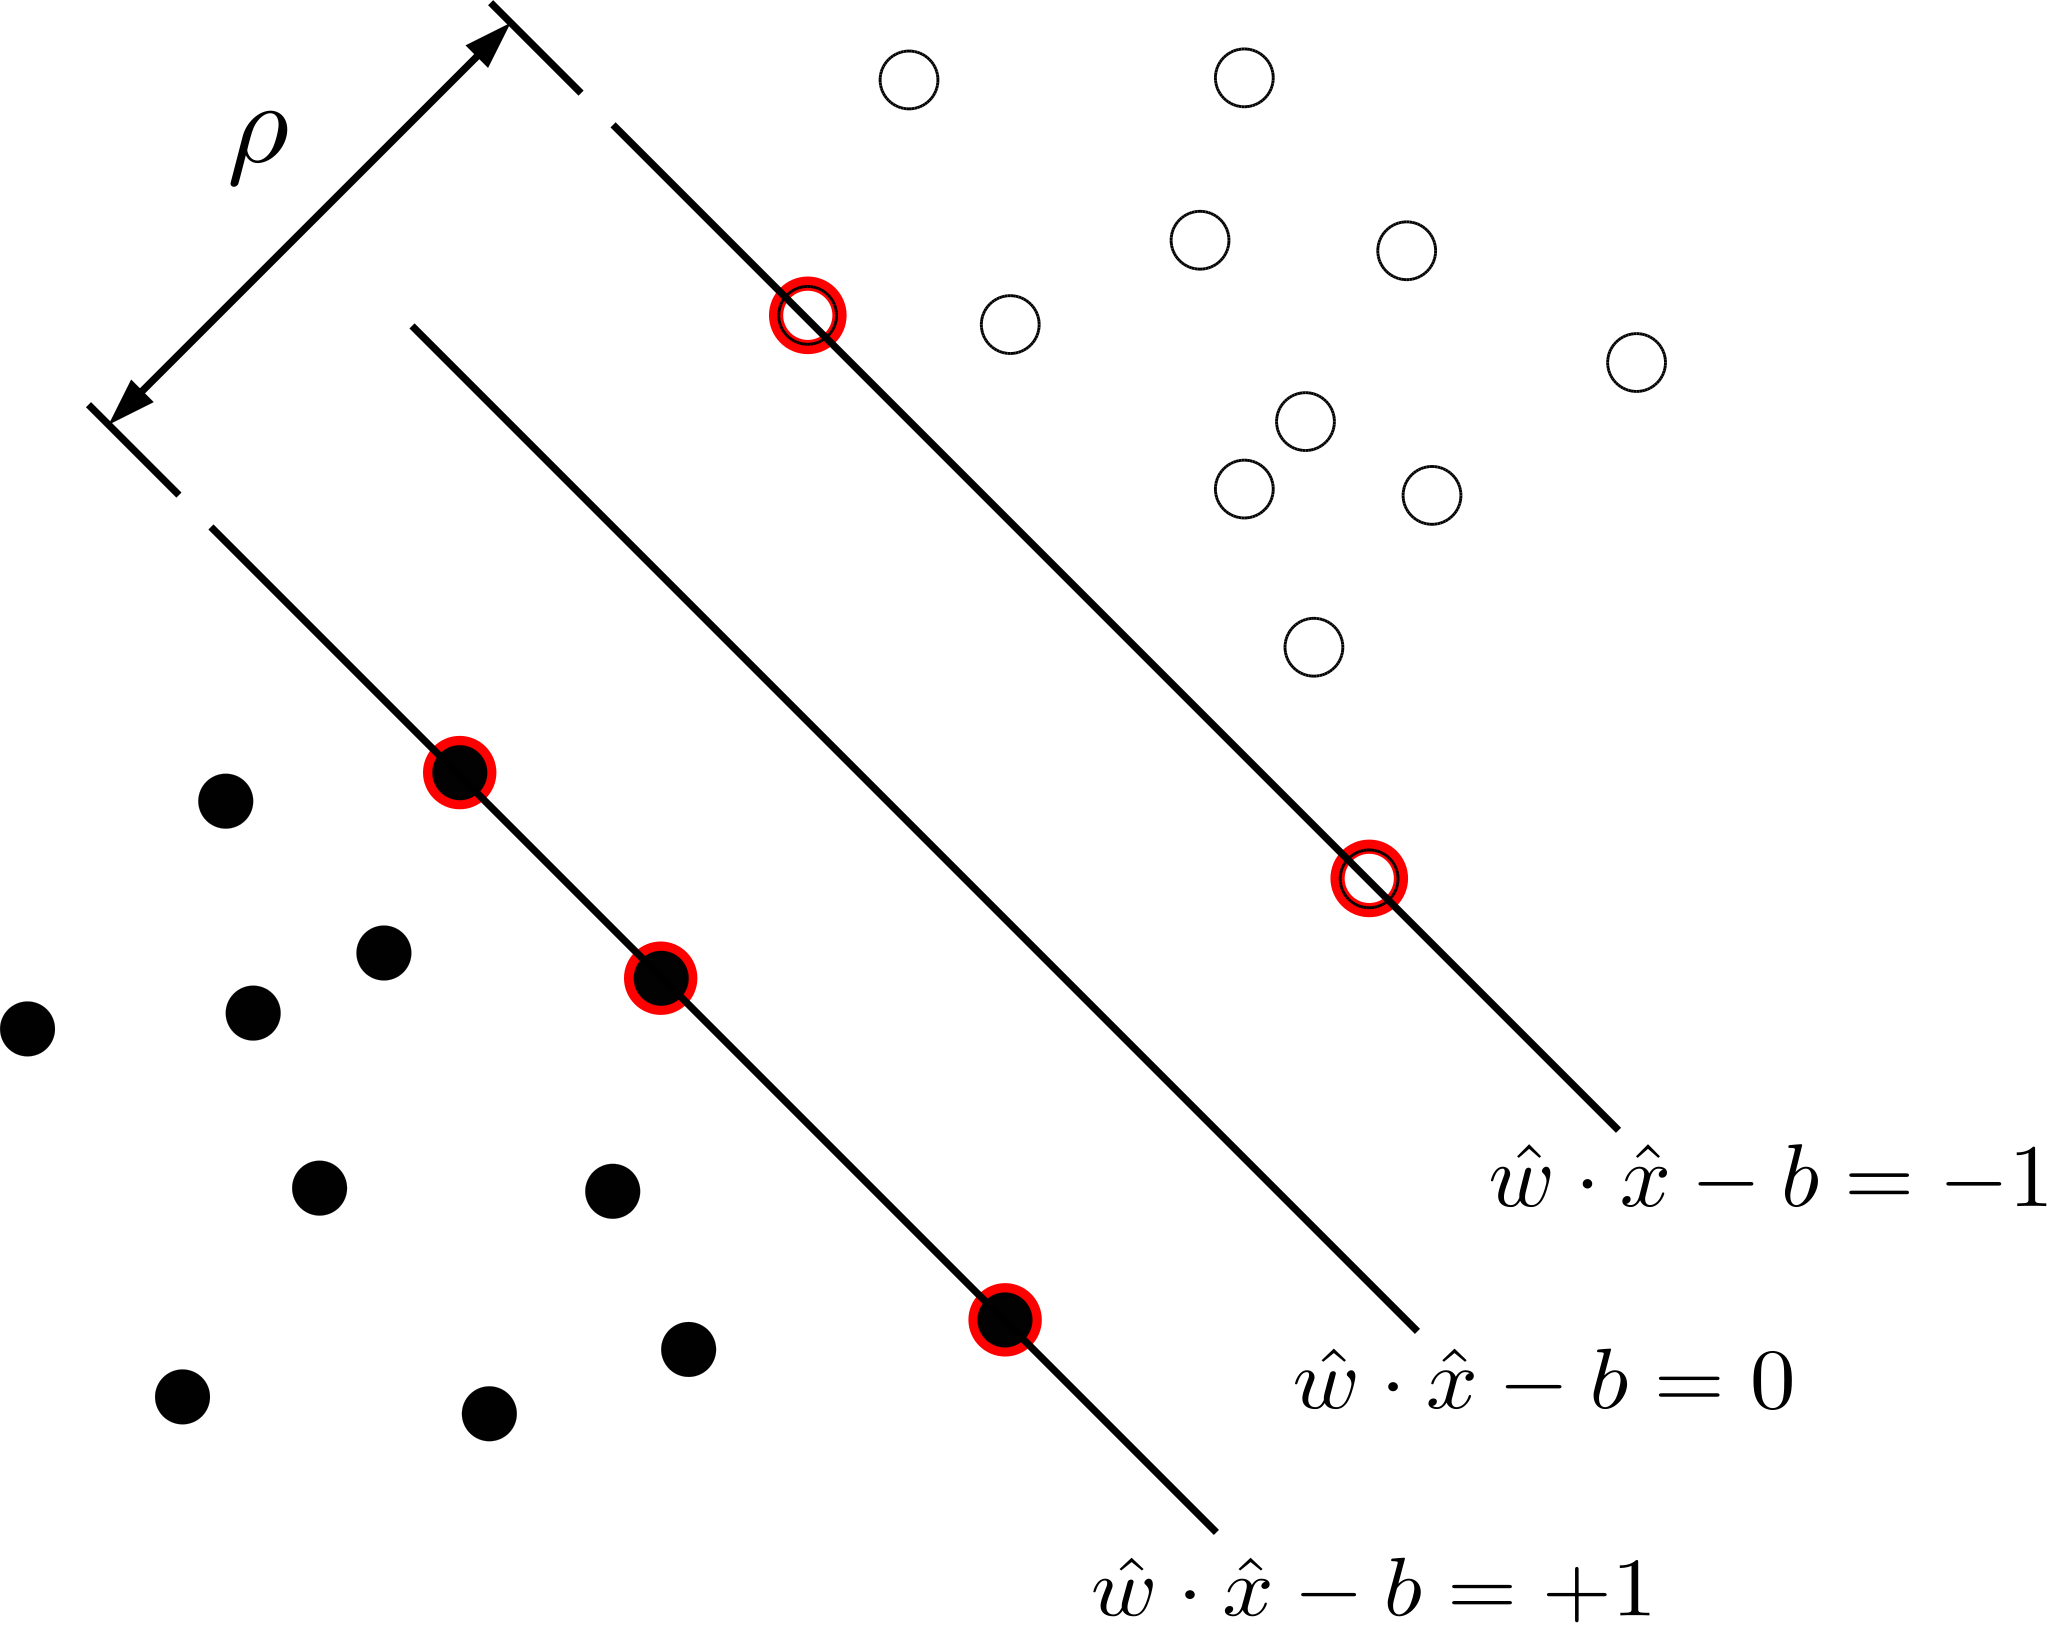
\includegraphics[width=0.65\linewidth]{img/SVM_margins}
	\caption{A hyperplane separating two classes with the maximum margin. The red highlighted points are the support vectors.
	}
	\label{fig:SVM_margins}
\end{figure} 

Formally, suppose that all the data satisfy the constraints

\begin{equation}
\vec{w}\cdot\vec{x}_i + b \geq +1 \text{   for   } y_i = +1,
\end{equation}
\begin{equation}
\vec{w}\cdot\vec{x}_i + b \leq +1 \text{   for   } y_i = -1,
\end{equation}
where $\vec{w}$ is the normal to the hyperplane, $\frac{|b|}{\|\vec{w}\|}$ is the perpendicular distance
from the hyperplane to the origin, and $\|\vec{w}\|$ is the Euclidean norm of $\vec{w}$. These two constraints can be expressed in compact form as:
\begin{equation}
\label{eq:svm_contraint}
y_i( \vec{w}\cdot\vec{x}_i + b)  \geq 1.
\end{equation}
The \textit{canonical hyperplane} is the hyperplane that separates the data and has maximal margin. 
%The training examples that satisfy the \ref{eq:svm_contraint} lie in the \textit{canonical hyperplanes} that satisfy the property
%\begin{equation}
%	\label{eq:canoncal_hyper}
%	\min_{\vec{x}_i \in X} |\vec{w}^T \cdot \vec{x}_i + b | = 1
%\end{equation}
The margin $\rho$ can be computed as the distance
between the two canonical hyperplanes:

\begin{equation}
\label{eq:dinstance_canocical}
\rho = \frac{1 - b}{\|\vec{w}\|} - \frac{- 1 - b}{\|\vec{w}\|} = \frac{2 }{\|\vec{w}\|} 
\end{equation}

Thus, we need to solve an optimisation problem, finding  the hyperplane that maximises the margin and ensures the classes are separable
\begin{equation}
\label{eq:svm_opt_problem}
\min_{\vec{w}_i, b} \frac{1}{2} \|\vec{w}\|^2 \textrm{ subject to } y_i( \vec{w}\cdot\vec{x}_i + b)  \geq 1.
\end{equation}
The problem can be expressed in the Lagrangian formulation:
\begin{equation}
\label{eq:lagrangian_svm_opt_problem}
\mathcal{L}(\vec{w}, b, \lambda) = \frac{1}{2} \|\vec{w}\|^2 + \sum_{i = 1}^{m} \lambda_i(1 -y_i ( \vec{w}\cdot\vec{x}_i + b))
\end{equation}
with Lagrange multipliers $\lambda_i \geq 0$ for each constraint in \ref{eq:svm_opt_problem}. The objective is then to minimize \ref{eq:lagrangian_svm_opt_problem} with respect to $\vec{w}$ and $b$ and simultaneously require that
the derivatives of $\mathcal{L}(\vec{w}, b, \lambda)$ with respect to all the $\lambda$ vanish. The advantage is twofold: the training vectors only appear as a scalar product among the vectors, and the constraints are easier to manage. 

With the formulation presented above, the SVM fails in some situation. In fact, there is no solution if samples can not be separated by a hyperplane. Moreover, although data are linearly separable the SVM may overfit to some outlier compromising system performance. For dealing with this type of problem, has been developed the soft margin SVM \cite{cortes95} which allows data points to lie within the margins. Introducing \textit{slack variables} $\xi_i$ into the constraints and penalize them in objective, the new problem becomes


\begin{equation}
%\begin{eqnarray}
\label{eq:slak_lagrangian_svm_opt_problem}
\min_{\vec{w}_i, b, \vec{\xi}} \frac{1}{2} \|\vec{w}\|^2 +  C\sum_{i = 1}^{m}\xi_i 
%\end{eqnarray}
\end{equation}
\begin{equation}\nonumber
\textrm{ subject to } y_i( \vec{w}\cdot\vec{x}_i + b)  \geq 1 - \xi_i \textrm{ and } \xi_i \geq 0 \textrm{ for } i = 1 \cdots m.
\end{equation}
The cost coefficient C > 0 is a hyper-parameter that specifies the misclassification penalty and is tuned by the user based on the classification task and dataset characteristics.
\paragraph{Non-Linear Support Vector Machines}
A way to solve the problem when data are not linearly separable, is to map the data on to a higher dimensional space and then to use a linear classifier in the higher dimensional space. This methods is referred to as ``the kernel trick '' that exploit the fact that the training data appears as a dot product between vectors in the Lagrangian formulation to from non-linear decision boundaries. Suppose to use a transformation $ \Phi:\vec{x} \to \phi(\vec{x}) $ to map every data sample into higher dimensional space, the dot product becomes $\phi(\vec{x}_i)^{T}\phi(\vec{x}_j)$. By the use of a kernel function 
\begin{equation}
K(\vec{x}_i,\vec{x}_j) = \langle\phi(\vec{x}_i), \phi(\vec{x}_j) \rangle ,
\end{equation}
it
is possible to compute the separating hyperplane without explicitly carrying out
the mapping into feature space. The classifier become:
\begin{equation}
f(\vec{x}) = \mbox{sign}(\sum_i \lambda_i y_i K(\vec{x}_i, \vec{x}_j) + b)
\end{equation}
The most popular kernel functions are:
\begin{itemize}
	\item Linear Kernel: 
	\begin{equation}
	K(\vec{x}_i,\vec{x}_j) = \langle\vec{x}_i, \vec{x}_j \rangle 
	\end{equation}
	
	\item Polynomial Kernel:  	  	 
	\begin{equation}
	K(\vec{x}_i,\vec{x}_j) = (\langle\vec{x}_i, \vec{x}_j \rangle)^d 
	\end{equation}
	\item Sigmoid Kernel: 
	\begin{equation}
	K(\vec{x}_i,\vec{x}_j) = tanh(\gamma\langle\vec{x}_i, \vec{x}_j \rangle -\theta ) 
	\end{equation}
	\item RBF Kernel: 
	\begin{equation}
	K(\vec{x}_i,\vec{x}_j) = \exp(-\frac{\|\vec{x}_i - \vec{x}_j \|}{2\sigma^2})  
	\end{equation}
\end{itemize}

Up to now the SVM algorithm for binary classification has been described. This algorithm can be extended to the multi-class case using the ``one vs all'' technique \cite{bishop06}.


\subsection{One-Class Support Vector Machines}
One-Class SVM (OCSVM) proposed by Sch{\"o}lkopf et al. \cite{scholkopf2000support} is the extension of the support vector machine to the case of unlabeled data that makes them useful for novelty detection problems. In the OCSVM, a new parameter $\nu$ 
that controls the trade-off between maximizing the distance of the hyperplane from the origin and the number of data points contained by the hyperplane has been introduced. To separate the data from the origin, the following quadratic program has to be solved:
\begin{equation}
%\begin{eqnarray}
\label{eq:ocsv_quadratic_problem}
\min_{\vec{w}_i, \vec{\xi}, \rho} \frac{1}{2} \|\vec{w}\|^2 +  \frac{1}{\nu l}\sum_{i = 1}^{m}\xi_i - \rho
%\end{eqnarray}S
\end{equation}
\begin{equation}\nonumber
\textrm{ subject to }\quad ( \vec{w}\cdot \phi(\vec{x}_i))  \geq \rho - \xi_i \textrm{ and } \xi_i \geq 0 \textrm{ for } i = 1 \cdots m.
\end{equation}
In fact, One-Class SVM consists in a discriminant function that takes the value $+1$ in a small region that captures the majority of the data points of a set and $-1$ outside that region \cite{scholkopf2000}. The discriminant function has the following expression:
\begin{equation}\label{eq:svm}
f(\mathbf{x}) = \mathop{\mathrm{sgn}} \left( \sum_{i} \alpha_i \cdot k(\mathbf{x}_i,\mathbf{x}) - \rho\right),
\end{equation}
where $ \vec{x}_i$ denotes the $i$-th support vector. The position of the hyperplane, thus, defines the region that represents normal data points. For each point $\textbf{x}$ that lies outside this region, the function $f( \vec{x})$ takes the value $-1$, whereas for point inside the region, it takes the value $+1$.
The terms $\lambda_i$ can be found by solving the solution to the dual problem:


The terms $\lambda_i$ can be found by solving the solution to the dual problem:
\begin{equation}
\min_{\lambda} \frac{1}{2} \sum_{ij}^{} K(\vec{x_i}, \vec{x_j}) 
\end{equation}
\begin{equation}\nonumber
\textrm{ subject to }\quad 0 \leq \lambda_i \leq \frac{1}{\nu l}\quad \textrm{ and }\quad \sum_{i}^{} \lambda_i = 1,
\end{equation}
where $\lambda_i$ is a Lagrange  multiplier and $l$ is the number of points in the  training dataset.
The term $\nu \in (0,1]$ is an hyperparameter of the algorithm that is determined on a validation set. 

The offset $\rho$ can be obtained from the Karush-Kuhn-Tucker (KKT) condition with the expression \cite{boyd2004convex}:
\begin{equation}
\rho = \sum_j \lambda_i k(\vec{x}_j,\vec{x}_i),
\end{equation}
which is satisfied for any $\lambda_i$ that is not at the upper or lower bound.



\section{Gaussian Mixture Model}
https://pdfs.semanticscholar.org/734b/07b53c23f74a3b004d7fe341ae4fce462fc6.pdf
A Gaussian Mixture Model (GMM) is a parametric probability density function represented as a weighted sum of Gaussian component densities. Generally, GMMs are used as a parametric model of the probability distribution of some features.  To estimate the parameter of GMM the algorithm Expectation-Maximization (EM) algorithm or Maximum A Posteriori (MAP)  are used starting from a well-trained prior model usually named Universal Background Model (UBM).
A Gaussian mixture model is a weighted sum of M component Gaussian densities as given by the equation
\begin{equation}
p(\vec{x, \lambda}) = \sum_{i = 1}^{M} w_i g(\vec{x} |\vec{\mu}_i, \vec{\Sigma}_i)
\end{equation}
where $\vec{x}$ is a D-dimensional features vector, $g (\vec{x} |\vec{\mu}_i), \vec{\Sigma}_i)$ are the components of the mixture and $w_i$ are the weight of each component. Each component of the mixture is a D-variate Gaussian density function expressed as
\begin{equation}
a
\end{equation}
\section{K-Nearest Neighbor}
\section{Deep Neural Network}
\subsection{Convolutional Neural Network}
\subsection{Autoencoder}
%\subsection{Siamese Neural Network}


